Dynamic memory allocation makes it possible for you to allocate additional space for your program to use from the \nameref{sub:heap}. We are going to look at two different examples of how to use dynamic memory allocation, both of which extend the Small DB program created in \cref{cha:more_data_types}. The first version will use a dynamically allocated array to allow the program to store a variable number of rows. Whereas, the second example will dynamically store each row, and link them together in memory. 

\subsection{Designing Small DB 2} % (fold)
\label{sub:designing_small_db_2}

\tref{tbl:small-db-2-prog} contains the extended description of the Small DB program that will be explored in this chapter. The main change is that in \cref{cha:more_data_types} the program only read in a fixed number of values. In this version the program will be able to respond to the user wanting to add or delete data stored in the program. In effect the program will store a \emph{variable} number of elements, with elements being added and removed by the user.

\begin{table}[h]
\centering
\begin{tabular}{l|p{10cm}}
  \hline
  \multicolumn{2}{c}{\textbf{Program Description}} \\
  \hline
  \textbf{Name} & \emph{Small DB 2} \\
  \\
  \textbf{Description} & Stores a number of values for the user. These values can be text (up to 7 characters), a whole number, or a real number. Each value entered is stored in a row with a unique identifier that will be assigned by the system. The first value will be assigned the id 0, the second will be assigned the id 1, and so on.\\
  & \\
  & The program will show the user a menu, and allow them to \textbf{add} new data to the program, \textbf{print} the data in the program, \textbf{delete} data from the program, or \textbf{quit}.\\
  & \\
  & \textbf{Add}: will read a value from the user and store it within the program. This data will be allocated a sequential id. \\
  & \\
  & \textbf{Print}: will print all of the values from the program, along with their types. \\
  & \\
  & \textbf{Delete}: this will ask the user to enter the id of the data they want to delete, and then search for this data in the program. If a row exists with this id, it is removed from the program.\\
  & \\
  & \textbf{Quit}: terminates the program. The menu will be repeatedly shown to the user until they decide to quit. \\
  \hline
\end{tabular}
\caption{Description of the Small DB program.}
\label{tbl:small-db-2-prog}
\end{table}

As before, the process to design and implement this program will follow a number of steps:
\begin{enumerate}
  \item \textbf{Analyse} the problem (understand it and associated tasks).
  \item \textbf{Design} the solution, its artefacts and control flow.
  \item \textbf{Implement} the design in code.
  \item \textbf{Test} the solution, compiling and running it to check it works as required.
\end{enumerate}

% subsection designing_small_db_2 (end)

\subsection{The Analysis Phase: Understanding Small DB 2} % (fold)
\label{sub:understanding_small_db_2}

The first task in any software development is to understand, as fully as you can, the requirements of the program, and the associated tasks and data. As this is an extension of the Small DB program from \cref{cha:more_data_types} most of that analysis has already been done. A number of tasks and data types were identified in the process of \nameref{sub:understanding_small_db}, and \nameref{sub:choosing_artefacts_for_small_db}. 

To successfully implement these new features you must first think about what is required of the new software. Then you can move on to think about how you can achieve these goals in your code.

As identified above, the new goal is to allow the user to enter a variable number of values. They need to be able to add and remove data as they wish. To achieve this a menu will need to be added that allows them to choose the action they want to perform next. From the menu the user will be able to choose to \textbf{add}, \textbf{print}, or \textbf{delete} data or to quit the program. These tasks give us hints about the kinds of functions and procedures we can add to achieve this.

As well as thinking about additional tasks, you should also see if there is additional data. Read over the description and see if you can identify any additional data that the user may need to either enter into the program, or get out of it.

At first glance there may not appear to be any new data needed by this program. After all it is still allowing the user to enter the same values that it did in \cref{cha:more_data_types}. There is, however, one additional kind of data that is hinted at in the description. There will be data associated with the \textbf{menu}. The program is likely to need to work with values associated with the options the user will be selecting. This can be modelled in the code, making it a better reflect the the concepts associated with the program.

% subsection understanding_small_db_2 (end)

\subsection{The Design Phase: Choosing artefacts and designing control flow} % (fold)
\label{sub:the_design_process_choosing_artefacts_for_small_db_2_and_designing_control_flow}

Once you have understood what is required, you need to set about designing the solution. This involves choosing the artefacts to create and use, and designing the control flow within the functions and procedures you create. This is all about making decisions, how will you structure this functionality? What control flow will enable this behaviour? The many decisions you make will define the overall design of the software.

This program already has an existing design, that needs to be extended. The data is described in the \emph{Data Dictionary} in \tref{tbl:dd-small-db}. An overview of the functions and procedure of the solution was shown in the structure chart in \fref{fig:small-db-struct}. These are a good starting point, and for the most part will require no changes. The new additions will build on top of these.

\subsubsection{Modelling the menu options} % (fold)
\label{ssub:modelling_the_menu_options}

Modelling the data should always be high on your priority list, so the first task can be to think about how the menu options can be modelled. The user needs to be able to select from \textbf{add}, \textbf{print}, \textbf{delete}, and \textbf{quit}. At later stages there may be more options, but at this point that is the list. 

If you think back to \cref{cha:more_data_types}, there are only three kinds of type you can use to model the data associated with a program: \textbf{records}, \textbf{unions}, and \textbf{enumerations}. These are the tools that are available to you to model your data. A \emph{record} has a number of values one for each field, a \emph{union} has one value with the type based on the field it was stored in, a \emph{enumeration} represents a list of options.

An \textbf{enumeration} is the obvious choice for modelling the list of options the user can choose from the menu. We can create a \texttt{Menu Option} type that has the values \texttt{ADD\_DATA}, \texttt{PRINT\_DATA}, \texttt{DELETE\_DATA}, and \texttt{QUIT}.

% subsubsection modelling_the_menu_options (end)

\subsubsection{Modelling the dynamic rows} % (fold)
\label{ssub:modelling_the_dynamic_rows}

One of the first processes that needs to be designed is the process to \texttt{Add a Row} to the data stored in the program. This can use the \texttt{Read Row} function that already exists to get the data from the user, so its focus is on allocating additional space for the row and determining the row's id.

A review of the code in the current Small DB program indicates that the row's index and its id were the same value, and \texttt{Main} was taking advantage of this. When \texttt{Main} called \texttt{Read Row}, it passed in \texttt{i} as the \texttt{id} for the new row. In effect, the value in \texttt{i} was being used as the index that looped over the elements of the array as it was being populated, and it was keeping track of the \texttt{id} value for the newly created rows. This is no longer going to be the case as the user can now add and delete rows. When they delete a row the index and the id will no longer linked, so one variable cannot track both values. A \texttt{\textbf{Next Row Id}} value needs to be kept somewhere.

The \texttt{\textbf{Next Row Id}} and the \textbf{\texttt{Rows}} data are associated. These values can be modelled as a single \texttt{\textbf{Data Store}} \textbf{record}, with each \texttt{Data Store} having fields for the \texttt{Next Row Id} and \texttt{Rows}. This will keep the relevant information together, and allow the code to work with these values as a group.

\begin{itemize}
  \item \texttt{Next Row Id} will be an integer, it will be assigned the value 0 at the start and have its value incremented each time a row is added. 
  \item \texttt{Rows} will be a dynamically allocated array of \texttt{Row} values.
\end{itemize}

\csection{ In C, another issue that needs to be resolved is the fact that there will now be a \emph{variable} number of rows in the program. The number of rows will also need to be recorded, and maintained as rows are added and deleted. A \texttt{\textbf{Row Count}} value can also be added to the \texttt{Data Store} record.

\ccode{}{}{topics/dynamic-memory/application/data-store.c}
}

\passection{Pascal has built in support for dynamic arrays. This means that it keeps track of the \texttt{Row Count} for you. The number of rows in a \texttt{Data Store} value can be determined by using the \texttt{Length} function with the \texttt{Data Store}'s \texttt{Rows} field.

\pascode{}{}{topics/dynamic-memory/application/DataStore.pas}
}

\tref{tbl:dd-small-db-2} shows the new data dictionary for Small DB 2. This includes the addition of the \texttt{Menu Option} enumeration and the \texttt{Data Store} record.

\begin{table}[htbp]
  \centering
  \begin{tabular}{|l|l|l|}
    \hline
    \textbf{Data} & \multicolumn{2}{c|}{\textbf{Details}}  \\ 
    \hline
    \multicolumn{3}{c}{} \\
    \hline
    \textbf{\texttt{Menu Option}} & \multicolumn{2}{p{10cm}|}{An \textbf{enumeration} with the following options:}\\
    \hline
    & \texttt{ADD\_DATA} & The user wants to add a row.\\
    \hline
    & \texttt{PRINT\_DATA} & The user wants to print all rows.\\
    \hline
    & \texttt{DELETE\_DATA} & The user wants to delete a row.\\
    \hline
    & \texttt{QUIT} & The user wants to quit.\\
    \hline
    \multicolumn{3}{c}{} \\
    \hline
    \textbf{\texttt{Row}} & \multicolumn{2}{p{11cm}|}{The \textbf{record/struct} from \tref{tbl:dd-small-db} that stores the row's \texttt{id}, \texttt{value}, and \texttt{kind}.}  \\
    \hline
    \multicolumn{3}{c}{} \\
    \hline
    \textbf{\texttt{Data Kind}} & \multicolumn{2}{p{11cm}|}{The \textbf{enumeration} from \tref{tbl:dd-small-db} representing the kind of value that can be stored in a row.}\\
    \hline
    \multicolumn{3}{c}{} \\
    \hline
    \textbf{\texttt{Column Value}} & \multicolumn{2}{p{11cm}|}{The \textbf{union} from \tref{tbl:dd-small-db} that stores either an integer, double, or text value.}\\
    \hline
    \multicolumn{3}{c}{} \\
    \hline
    \textbf{\texttt{Data Store}} & \multicolumn{2}{p{10cm}|}{A \textbf{record} to store row data with the following fields:}\\
    \hline
    & \texttt{Next Row Id} & The id value of the next row to be added.\\
    \hline
    & \texttt{Rows} & A dynamically allocated array of \texttt{Row} values.\\
    \hline
    & \texttt{Row Count} & The number of rows in the \texttt{Data Store}. (C Only)\\
    \hline

  \end{tabular}
  \caption{Data Dictionary for Small DB 2}
  \label{tbl:dd-small-db-2}
\end{table}

% subsubsection modelling_the_dynamic_rows (end)

\subsubsection{Designing Small DB 2's Structure} % (fold)
\label{ssub:designing_small_db_2_s_structure}

The next step is to choose the functions and procedures that need to be created or used to implement this program. Once again, this can build on the structure implemented in Small DB, as shown in \fref{fig:small-db-struct}. This included the code needed to read a row from the user, and to output the row to the Terminal.

\begin{figure}[p]
   \centering
   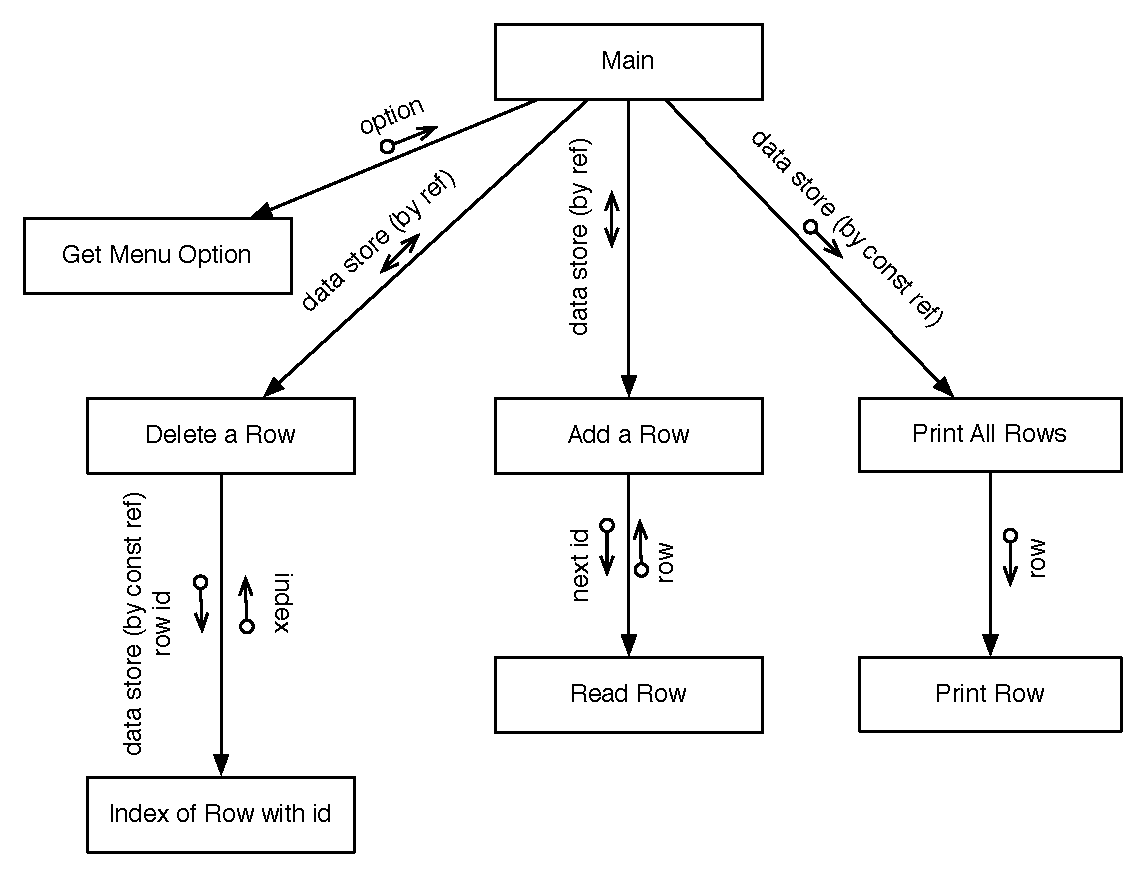
\includegraphics[width=0.90\textwidth]{./topics/dynamic-memory/diagrams/SmallDB2Structure} 
   \caption{Structure chart for Small DB 2}
   \label{fig:small-db-2-struct}
\end{figure}

Small DB 2 needs to add some additional functionality to this program. The following list shows the tasks that need to be coded, and the functions or procedures that will code their behaviour. This is shown in the Structure Chart in \fref{fig:small-db-2-struct}.

\begin{itemize}
  \item Show the menu to the user, and get the option they want to perform (\texttt{Get Menu Option} function).
  \item Add a row to the data managed in the program (\texttt{Add a Row} procedure).
  \item Print all of the rows (\texttt{Print All Rows} procedure).
  \item Delete a row from the data managed by the program (\texttt{Delete a Row} procedure).
\end{itemize}

In Small DB the logic for \texttt{Print all Rows} was coded into \texttt{Main}. This logic can be moved from there into its own procedure. The control flow for the other functions and procedures will need to be designed.

% subsubsection designing_small_db_2_s_structure (end)

\subsubsection{Control flow for \texttt{Get Menu Option}} % (fold)
\label{ssub:control_flow_for_get_menu_option}

The code for \texttt{Get Menu Option} should be fairly simple. The basic actions it needs to perform will be:
\begin{enumerate}
  \item Output the text showing the list of options to the Terminal.
  \item Read a number from the user, making sure it is in the range of the list of options (1 to 4).
  \item Return the value of the option selected as a \texttt{Menu Option} value.
\end{enumerate}

The first part of this process will involve a sequence of output commands, displaying the different text to the Terminal. The code to read a number from the user will need a standard \emph{validation} loop, repeatedly asking them to enter a number until they enter one between 1 and 4. The final part can use a \nameref{sub:case_statement} to return the correct result from the function.

% subsubsection control_flow_for_get_menu_option (end)

\subsubsection{Control flow for \texttt{Add a Row}} % (fold)
\label{ssub:control_flow_for_add a row}

The process for adding a row will involve the following steps, as shown in \lref{lst:add_row}:
\begin{enumerate}
  \item Record the next row id, and then increase the \texttt{Next Row Id} in the \texttt{Data Store}.
  \item Increase the memory allocated to the \texttt{Data Store}'s \texttt{Rows} (and the Row Count, in C), and store the \texttt{Row} read from the user into this newly allocated memory.
\end{enumerate}

\pseudocode{lst:add_row}{Pseudocode for the \texttt{Add a Row} procedure}{topics/dynamic-memory/application/AddRow.txt}
% subsubsection control_flow_for_add a row (end)

\subsubsection{Control flow for \texttt{Delete a Row}} % (fold)
\label{ssub:control_flow_for_}

Deleting an element out of an array is a common task, but one that will require you to perform all of the hard work. Remember that arrays are \emph{contiguous blocks of memory}, so technically you cannot delete an element from the middle of this array. You can only remove the last element. There are three options for how this can be achieved, as shown in \fref{fig:delete-illustration}. All of the options involve moving data, and then resizing the dynamically allocated array to have one fewer element than before. The different options involve copying different pieces of data to free the last slot so that its allocation can be released.

\begin{enumerate}
  \item Only copy the last element over the element to be deleted. This is the fastest, but the order of the elements is not preserved. If this is important then you cannot use this approach.
  \item The second option is to copy the value of each element in the array back over the previous element. This maintains the order of the elements, but takes more time as you have to copy all of the values after the element being deleted back one spot.
  \item A faster option is to take advantage of the fact the array is stored as a contiguous block, and to perform a bulk move/copy of the memory past the element. In effect, you can copy all of the elements with one request and take advantage of the hardware which is optimised for this kind of task.
\end{enumerate}

\begin{figure}[h]
   \centering
   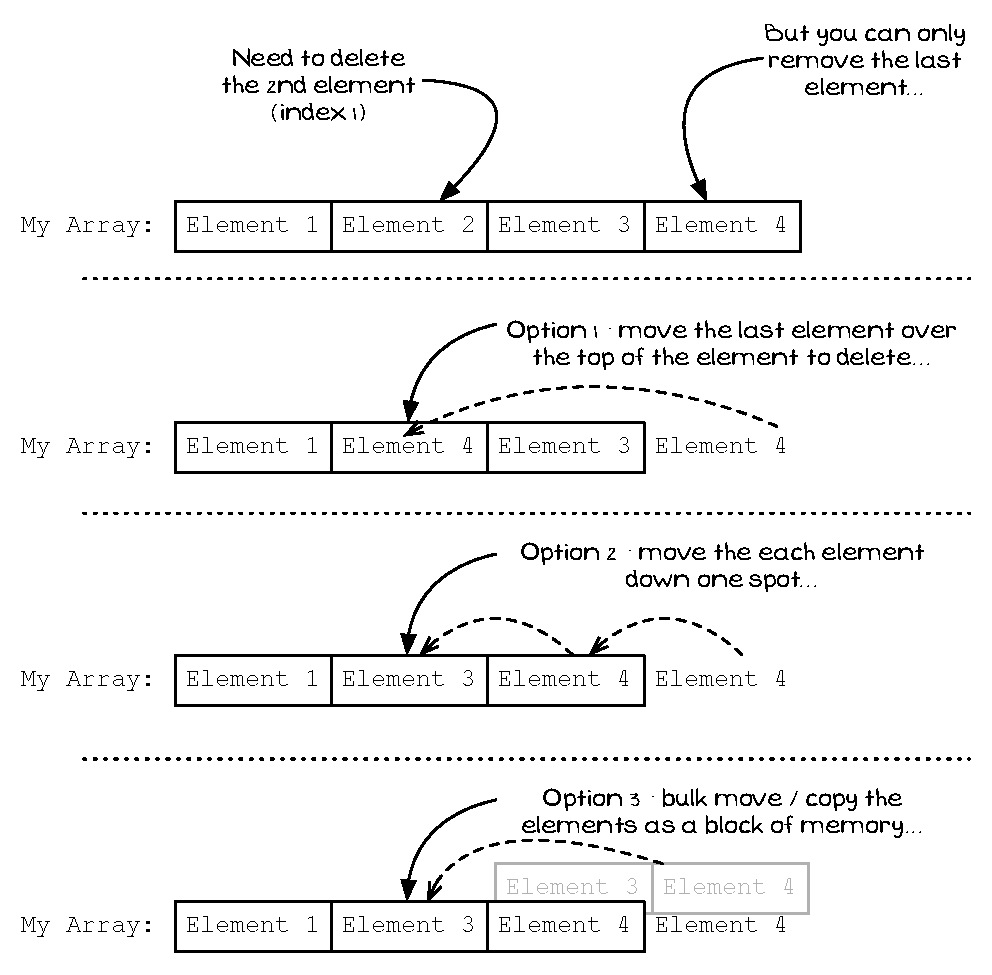
\includegraphics[width=0.87\textwidth]{./topics/dynamic-memory/diagrams/DeleteIllustration} 
   \caption{Options for deleting an element from an array}
   \label{fig:delete-illustration}
\end{figure}

\fref{fig:delete-a-row-flow} shows the flowchart of the process for deleting a node from the \texttt{Rows} array using Option 2. This option has been chosen as it helps demonstrate the use of the elements of the array, as well as working with the dynamic memory. 

The implementation of this option also demonstrates a frequently seen pattern when working with two consecutive elements of an array. In this case one element is being copied over another, but many algorithms will require you to work with two elements at a time. Each time through the loop, this code will access the $i^{th}$ element and its neighbour, the $(i+1)^{th}$ element.\footnote{An alternative version of this is to start 1 element past the first element you want to interact with, and use the $i^{th}$ element and the previous element, the $(i-1)^{th}$ element.} This means the loop needs to go from a starting element, to the \textbf{second last} element of the array. If \texttt{i} looped to the \emph{last element} of the array then \texttt{i+1} would attempt to access an element past the end of the array.

\begin{figure}[htbp]
   \centering
   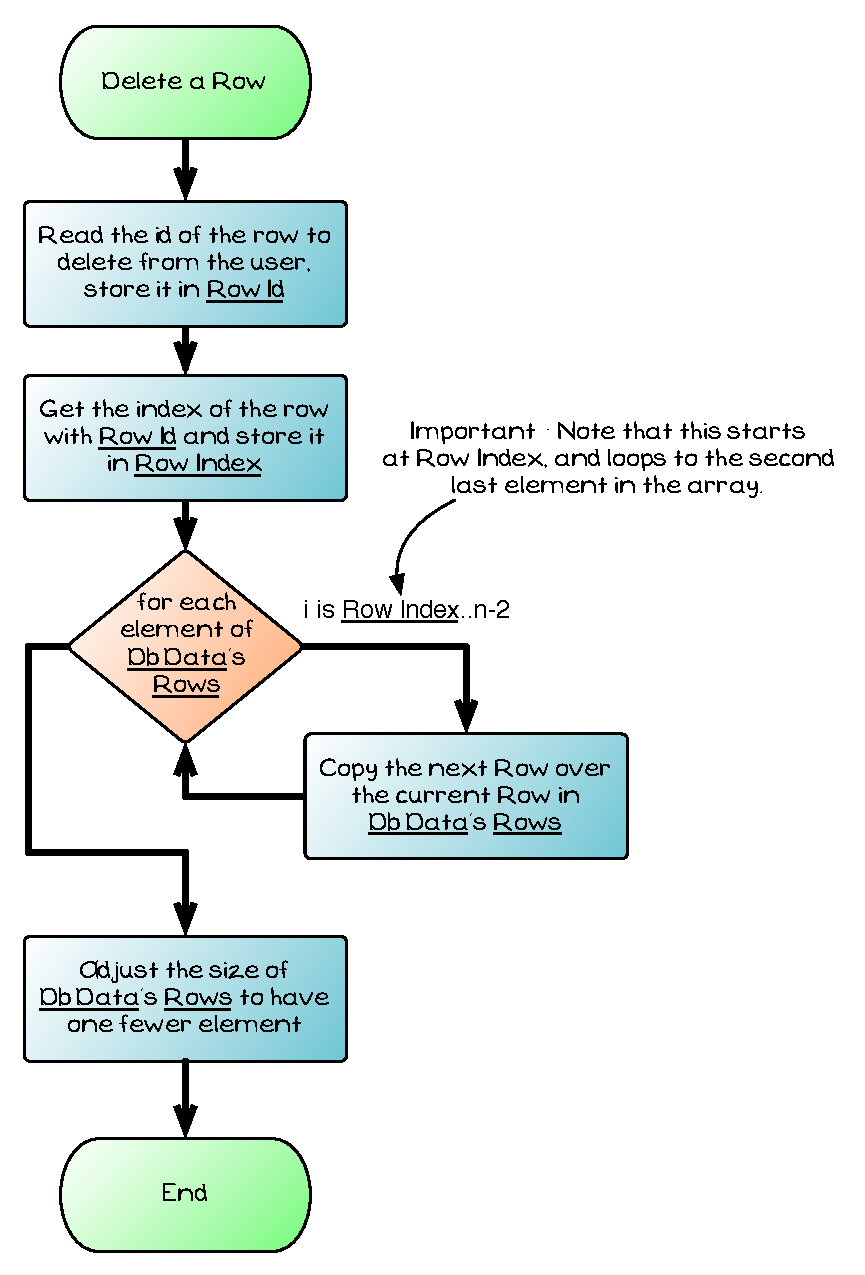
\includegraphics[width=0.7\textwidth]{./topics/dynamic-memory/diagrams/DeleteFlow} 
   \caption{Flowchart describing the process for deleting a row with a given id}
   \label{fig:delete-a-row-flow}
\end{figure}


% subsubsection control_flow_for_ (end)

\subsubsection{Control flow for \texttt{Index of Row with Id}} % (fold)
\label{ssub:control_flow_for_index of row with id}

The \texttt{Index of Row with Id} function will search a \texttt{Data Store}'s \texttt{Rows} for the index of the \texttt{Row} with the \texttt{Id} it is searching for. This is used by the \texttt{Delete a Node} procedure so that it can find the index of the row it needs to delete.

This is implemented using a standard \textbf{search pattern}. This pattern involves looping over all of the elements in the array, and \emph{for each} element checking `\emph{Is this the element I am after?}'. When a match is found the search can end, as can the function. This can be implemented using the appropriate \nameref{sub:exit} statement for the language, with  the function returning the index of the row it found, in this case. However, if the loop gets to the end of the array without finding a match, then there is no element in the array that matches the search and the function can return a value that indicates no match was found, in this case the index \texttt{-1} is returned as this cannot be a valid index. The flowchart illustrating these steps is shown in \fref{fig:index-of-row-flow}.

\begin{figure}[h]
   \centering
   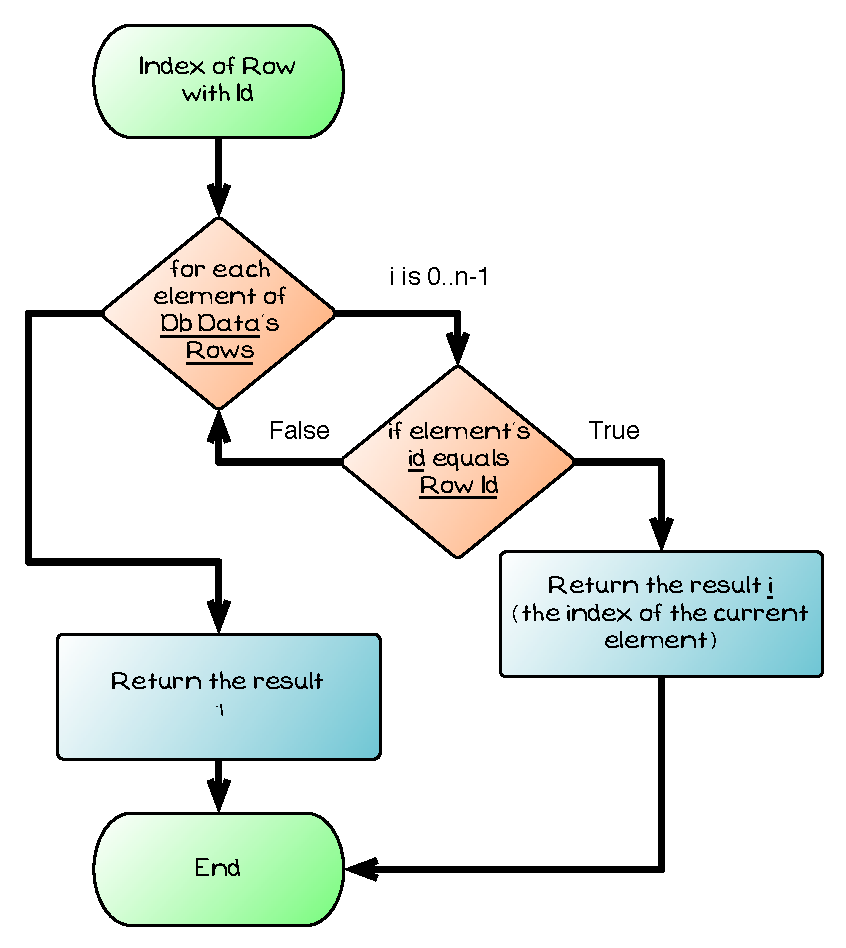
\includegraphics[width=0.75\textwidth]{./topics/dynamic-memory/diagrams/IndexOfRowFlow} 
   \caption{Flowchart describing the process for finding the index of a row with a given id}
   \label{fig:index-of-row-flow}
\end{figure}


% subsubsection control_flow_for_index of row with id (end)

\subsubsection{Control flow for \texttt{Main}} % (fold)
\label{ssub:control_flow_for_main}

\texttt{Main} is the last remaining procedure. The implementation of this will require you to declare a \texttt{Data Store} variable that will be manipulated by the other procedures previously discussed. This will need to be initialised with no elements in its \texttt{Rows}, and other a \texttt{Next Row Id} of 0.

The control flow of Main will involve a \nameref{sub:post_test_loop} that will repeat code until the user chooses to quit. Within the loop \texttt{Main} can get the option the user wants to perform by calling the \texttt{Get Menu Option} function, can then use a \nameref{sub:case_statement} to run either the \texttt{Add a Row} procedure, the \texttt{Print all Rows} procedure, or the \texttt{Delete a Row} procedure.

% subsubsection control_flow_for_main (end)

\clearpage
\subsection{The Implementation Phase: Writing the code for Small DB 2} % (fold)
\label{sub:writing_the_code_for_small_db_2}

The following two sections, \sref{sec:dynamic_memory_allocation_in_c} \nameref{sec:dynamic_memory_allocation_in_c} and  \sref{sec:dynamic_memory_allocation_in_pascal} \nameref{sec:dynamic_memory_allocation_in_pascal}, contain a description of the syntax needed to code dynamic memory allocation in the C and Pascal programming languages. Use this information to write the code for Small DB 2, and other programs.

% subsection writing_the_code_for_small_db_2 (end)

\subsection{The Testing Phase: Compiling and running Small DB 2} % (fold)
\label{ssub:the_testing_phase_compiling_and_running_small_db_2}

Whenever you work with dynamic memory allocation, you need to spend a good proportion of your time checking that your solution is working. This is now an interactive program, so you can test multiple things each execution. The following are some of the aspects that you should test in this program:

\begin{itemize}
  \item Test the basic functionality:
  \begin{itemize}
    \item Can you add new rows?
    \item Can you delete a row?
    \item Can you print the rows?
    \item Are you able to quit the program?
  \end{itemize}
  \item Test for potential issues related to memory allocation:
  \begin{itemize}
    \item Try deleting the first row, the last row, and a non-existent row.
    \item Delete all of the rows.
    \item Print when there are no rows.
    \item Delete and then add, delete all rows then add, etc.
  \end{itemize}
\end{itemize}

Think about the places where you may have made a mistake, and test to check that you can not cause the program to crash. 

\mynote{
There \textbf{is} a bug in the current design, as presented in this chapter. If you run these tests you should be able to find the bug, which has the potential to cause the program to crash. See if you can locate the bug, correct it, and implement the required fix. Like most bugs the fix only requires a small change, so think carefully about what is required.
}

% subsection the_testing_phase_compiling_and_running_small_db_2 (end)

% subsection the_design_process_choosing_artefacts_for_small_db_2_and_designing_control_flow (end)

\clearpage
\subsection{Designing Linked Small DB 2} % (fold)
\label{sub:designing_linked_list}

Arrays are only one way of dynamically allocating space for a program. In an array the elements are allocated in a contiguous block, each element next to the previous one. This structure is good when you want to access an element based on its position, but operations like delete and insert can be tricky as you need to move elements around to make or remove space.

An alternative to the array, is to dynamically allocate space for each value individually, and to use pointers to record their locations. The general structure is called a \textbf{Linked List}, and we can use this to manage the \texttt{Row}s in the linked version of the Small DB 2 program.

\fref{fig:array-vs-linked} shows the difference between how the rows are stored in the previous array version of Small DB 2, and the linked version we will now explore. In the array version, each \texttt{Row} is stored next to the previous one in an array. With this version you can use an index value to access the middle elements of the array quickly, but it is slower to delete or insert elements. 

The linked version of Small DB 2 is made up of nodes (the \texttt{Row}s) that each store the data and a \emph{link} (pointer) to the \texttt{next} node in the list. In this version the \texttt{Row}s are not stored next to each other, so you cannot use an index to calculate the position of any one element. Instead you need to start at the first element, and work your way through the list one element at a time using the \texttt{next} pointer to move from the current node to the next node of the list. Inserting or deleting elements of the list can be much faster as the \emph{links} can be adjusted to introduce new elements, or remove existing one from the list.

\begin{figure}[htbp]
   \centering
   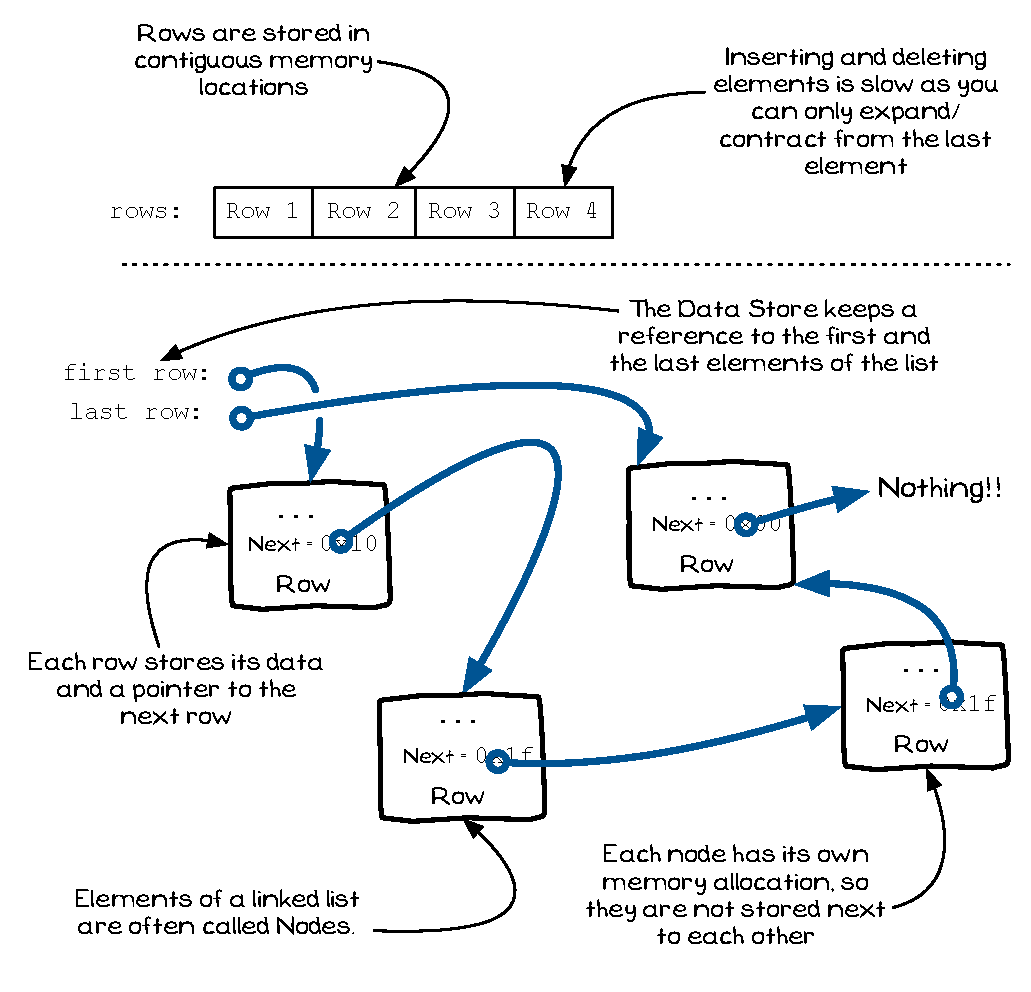
\includegraphics[width=0.85\textwidth]{./topics/dynamic-memory/diagrams/ArrayVsList} 
   \caption{Illustration of memory layout for Array and Linked versions of Small DB 2}
   \label{fig:array-vs-linked}
\end{figure}

% subsection designing_linked_list (end)

\subsection{The Design Place: Designing Linked Small DB 2} % (fold)
\label{sub:the_design_place_designing_linked_small_db_2}

The linked version of the Small DB 2 program is an alternative implementation for the same program developed in \sref{sub:designing_small_db_2}. This means that the information from the analysis phase is still valid, and can be used to inform what must be done in this program. Similarly, the testing strategies developed will also be valid so when the design and implementation are complete you can test it in the same way as the previous program.

The parts that do need to change will be the \textbf{design} and \textbf{implementation}. The design needs to structure the data differently, and this will impact on the structure of the code as well. The first step, therefore, is to design the new structure for the data and then to use this to determine the new structure for the code.

\subsubsection{Modelling the links in data} % (fold)
\label{ssub:modelling_the_links_in_data}

\tref{tbl:dd-linked-small-db-2} shows the new data dictionary for the linked version of the Small DB 2 program. Most of the changes relate to the \texttt{Data Store} record. This used to store all of the rows in a dynamically allocated array. Now, in the linked version, the \texttt{Data Store} includes two pointers: one pointing to the first \texttt{Row}, the other pointing to the last \texttt{Row}. Only the first of these two is actually required, but the pointer to the last \texttt{Row} will make some tasks easier.

The \texttt{First Row} pointer, points to the first \texttt{Row} value allocated on the heap. Tasks like \texttt{Print all Rows} will use this pointer to start looping through the \texttt{Row}s. The \texttt{Last Row} pointer exists to make it easier to add new \texttt{Row}s to the \texttt{Data Store}. New \texttt{Row}s are added to the end of the list, and the \texttt{Last Row} pointer means you can get to the end of the list without first having to loop through each node.

\begin{table}[h]
  \centering
  \begin{tabular}{|l|l|l|}
    \hline
    \textbf{Data} & \multicolumn{2}{c|}{\textbf{Details}}  \\ 
    \hline
    \multicolumn{3}{c}{} \\
    \hline
    \textbf{\texttt{Row}} & \multicolumn{2}{p{11cm}|}{The \textbf{record/struct} from \tref{tbl:dd-small-db} that stores the row's \texttt{id}, \texttt{value}, and \texttt{kind}. This now also has an additional field to point to the location of the next \texttt{Row}}  \\
    \hline
    & \texttt{Next} & A pointer to the next \texttt{Row}.\\
    \hline
    \multicolumn{3}{c}{} \\
    \hline
    \textbf{\texttt{Data Kind}} & \multicolumn{2}{p{11cm}|}{The \textbf{enumeration} from \tref{tbl:dd-small-db} representing the kind of value that can be stored in a row.}\\
    \hline
    \multicolumn{3}{c}{} \\
    \hline
    \textbf{\texttt{Column Value}} & \multicolumn{2}{p{11cm}|}{The \textbf{union} from \tref{tbl:dd-small-db} that stores either an integer, double, or text value.}\\
    \hline
    \multicolumn{3}{c}{} \\
    \hline
    \textbf{\texttt{Menu Option}} & \multicolumn{2}{p{11cm}|}{An \textbf{enumeration} from \tref{tbl:dd-small-db-2} with options for adding a row, printing all rows, deleting a row, or quitting the program.}\\
    \hline
    \multicolumn{3}{c}{} \\
    \hline
    \textbf{\texttt{Data Store}} & \multicolumn{2}{p{10cm}|}{A \textbf{record} to store row data with the following fields:}\\
    \hline
    & \texttt{Next Row Id} & The id value of the next row to be added.\\
    \hline
    & \texttt{First Row} & A pointer to the first \texttt{Row} in the \texttt{Data Store}.\\
    \hline
    & \texttt{Last Row} & A pointer to the last row in the \texttt{Data Store}.\\
    \hline

  \end{tabular}
  \caption{Data Dictionary for Linked version of Small DB 2}
  \label{tbl:dd-linked-small-db-2}
\end{table}

One tricky aspect of the linked \texttt{Row}s, is that the \texttt{Row} must include a pointer to a \texttt{Row}. In most cases the compiler requires that the thing you are using is declared before its use. Here that is not possible, the declaration of the row must include the point to the row which is still being declared. Each language caters for this in its own way, the tricks for doing this in C are shown in \fref{clst:row-node}, the Pascal version is shown in \fref{paslst:row-node}.

\begin{figure}[p]
  \csection{The following code shows how the new \texttt{Data Store} and \texttt{Row} structures can be implemented in C. The one trick here is that you must use the \texttt{struct} name of the \texttt{Row} when declaring the \texttt{next} field. This is because C has not yet encountered the type name for the \texttt{Row}, so you need to use its alternate name.

    \ccode{}{}{topics/dynamic-memory/application/linked-data-store.c}
  }
  \caption{C code for declaring the \texttt{Row}, with a next pointer}
  \label{clst:row-node}
\end{figure}
\begin{figure}[p]
  \passection{The following code shows how the new \texttt{Data Store} and \texttt{Row} structures can be implemented in Pascal. The trick here is to declare an alias for the \texttt{RowPtr} (a pointer to a Row) before the \texttt{Row} declaration, but in the same type declaration part.

    \pascode{}{}{topics/dynamic-memory/application/LinkedDataStore.pas}
  }
  \caption{Pascal code for declaring the \texttt{Row}, with a next pointer}
  \label{paslst:row-node}
\end{figure}

% subsubsection modelling_the_links_in_data (end)
\clearpage
\subsubsection{Reviewing the structure for the linked version of Small DB 2} % (fold)
\label{ssub:reviewing_the_structure_for_the_linked_version_of_small_db_2}

The overall structure for Small DB 2 will not change much, as the basic actions the program needs to complete remain the same. The only real change is that the \texttt{Index of Row with ID} function is no longer required, as indexes no longer serve as a means of accessing the \texttt{Row} values in the \texttt{DataStore}. The updated version of the Structure Chart is shown in \fref{fig:linked-small-db-2-struct}.

\begin{figure}[htbp]
   \centering
   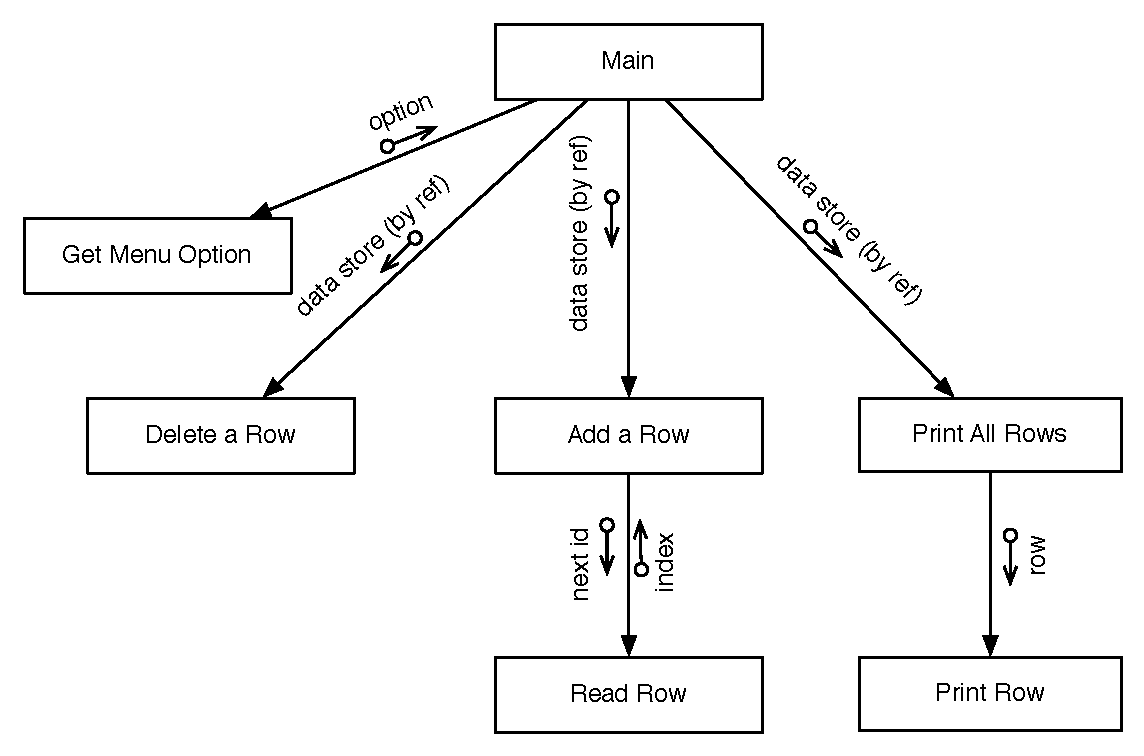
\includegraphics[width=0.90\textwidth]{./topics/dynamic-memory/diagrams/LinkedSmallDB2Structure} 
   \caption{Structure chart for the Linked version of Small DB 2}
   \label{fig:linked-small-db-2-struct}
\end{figure}

% subsubsection reviewing_the_structure_for_the_linked_version_of_small_db_2 (end)
\clearpage
\subsubsection{Adding a Row to the linked version of Small DB 2} % (fold)
\label{ssub:adding_a_row_to_the_linked_version_of_small_db_2}

The first activity that can be examined in detail is the \texttt{Add a Row} procedure. This will need to create a new \texttt{Row} value, and have it added to the end of the list. To start with, let us have a look at how this should work conceptually.

\fref{fig:add-node-1} shows an illustration of the add process for the first row. At the start the code has a single \texttt{Data Store} value, this will be \texttt{Db Data} from within the \texttt{Main} procedure. When the program start the data store will need to have its \texttt{First Row} and \texttt{Last Row} fields initialised to point to \emph{Nothing}. This indicates that there is no first row, or last row in the \texttt{Data Store} at this stage.

When a new Row is added the first step is to allocate space for it on the heap, and then to read the user's input into that space (using \texttt{Read Row}). As this \texttt{Row} will be added to the end of the \texttt{Data Store}, its \texttt{Next} field can be set to \emph{Nothing} to indicate that there are no more \texttt{Row} values after this one. 

\begin{figure}[htbp]
   \centering
   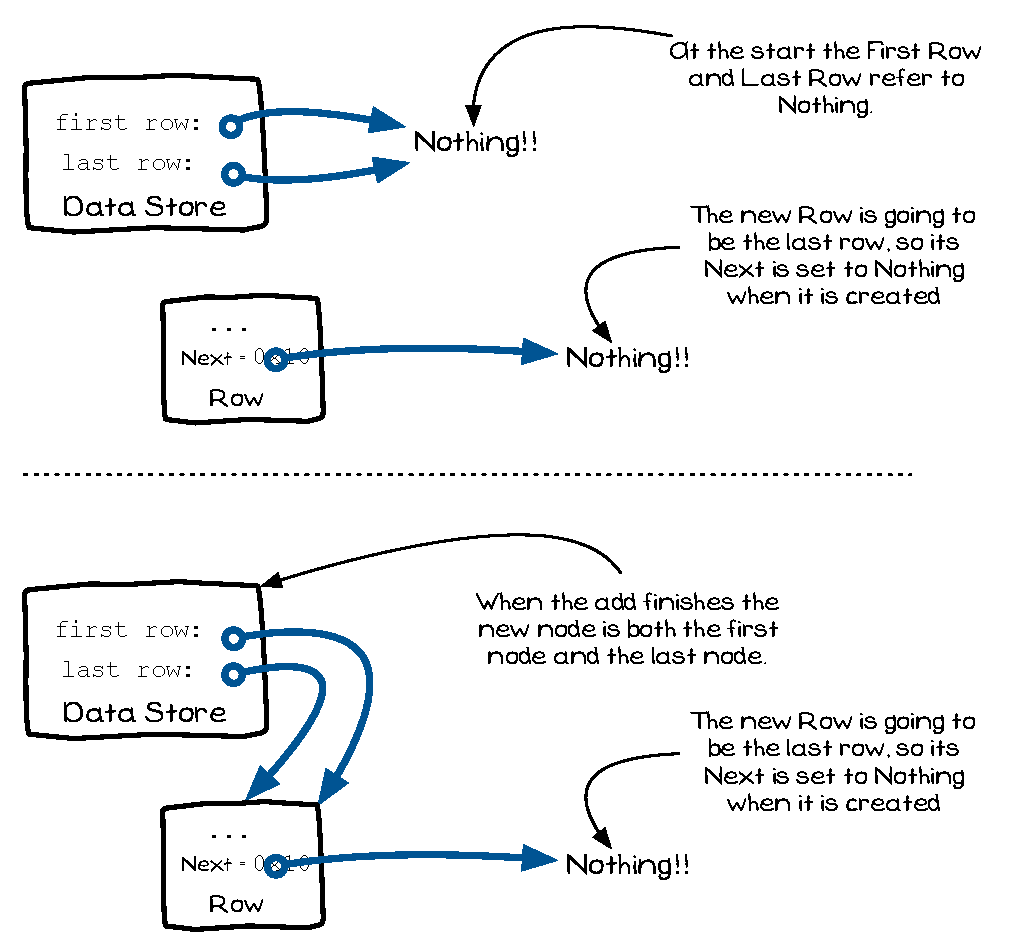
\includegraphics[width=0.80\textwidth]{./topics/dynamic-memory/diagrams/AddNode1} 
   \caption{The first Row becomes the start and end of the List}
   \label{fig:add-node-1}
\end{figure}

The code for \texttt{Add a Row} now needs to link this new \texttt{Row} into those already in the \texttt{Data Store}. This is where it checks to see if there is a \texttt{Row} value currently referred to be the \texttt{last row} of the \texttt{Data Store} value. As this refers to \emph{Nothing} at this point, the code takes a branch that sets the \texttt{first row} and the \texttt{last row} both to refer to the newly created \texttt{Row} value. At this point, the new \texttt{Row} is both the first and the last row in the \texttt{Data Store.}

\clearpage
Most the time when you add a new row it will not be the first one in the list. Typically, you will need to add the row to the existing rows in memory. This involves updating the current \texttt{last row} so that its \texttt{next} points to the newly created row, and then you can change the \texttt{Data Store}'s \texttt{last row} to point to it as well. This is shown in \fref{fig:add-node-2}, with the whole pseudocode shown in \lref{lst:add_linked_row}.

\begin{figure}[htbp]
   \centering
   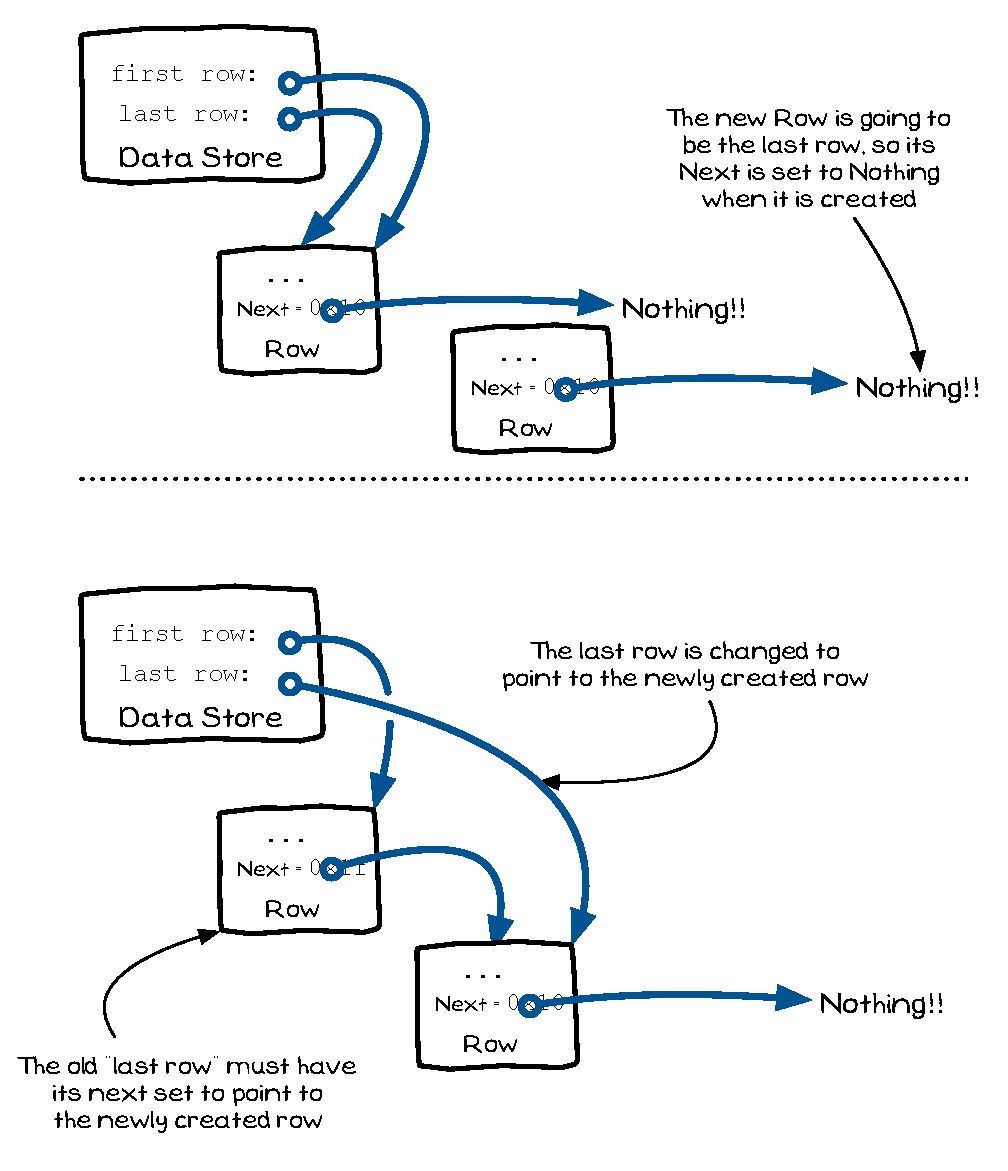
\includegraphics[width=0.80\textwidth]{./topics/dynamic-memory/diagrams/AddNode2} 
   \caption{When a new row is added, it becomes the new last row, and the old last node points to it}
   \label{fig:add-node-2}
\end{figure}

\begin{figure}[p]
  \pseudocode{lst:add_linked_row}{Pseudocode for the \texttt{Add a Row} procedure in the linked version of Small DB 2}{topics/dynamic-memory/application/AddLinkedRow.txt}  
\end{figure}

\begin{figure}[p]
  \mynote{
  \begin{itemize}
    \item Step 3 of \lref{lst:add_linked_row} allocates space on the heap for the row data, and stores a pointer to it in \texttt{New Row}.
    \item Step 6 checks if this is the first \texttt{Row} in the \texttt{Data Store}.
    \item Step 9 reads \texttt{Db Data}'s \texttt{Last Row} pointer, then follows it to the \texttt{Row}, so that it can store a value in that \texttt{Row}'s \texttt{Next} field.
  \end{itemize}
  }
\end{figure}

% subsubsection adding_a_row_to_the_linked_version_of_small_db_2 (end)

\clearpage
\subsubsection{Printing all rows in the linked version of Small DB 2} % (fold)
\label{ssub:printing_all_rows_in_the_linked_version_of_small_db_2}

The code in \texttt{Add a Row} will enable you to create a list of any length. Each row is linked in by changing the old \texttt{last row} to point to the newly created row, and then the \texttt{last row} of the \texttt{Data Store} is updated. This is all very nice, but now that you have the data within the program how do you use it?

As with an array, the think that you need to determine is how to perform some action \emph{for each} node in the list. There is no index that you can use to access the Nodes, so the standard \nameref{sub:for_loop} is not going to be of assistance. Instead, what you need to do is to iterate through the list by following the \texttt{next} pointers in each \texttt{Row}.

The standard pseudocode for looping through \emph{each} node in a list is shown in \lref{lst:iterate-linked-list}. The main idea is that you can have a \texttt{current} node that you are processing. Then, to get to the next node you follow \texttt{current} pointer and read the \texttt{next} field. The result is then a pointer to the next node in the list and can be stored as the \texttt{current} node. This process can then be repeated \textbf{while} \texttt{current is not nothing}. This process is shown in \fref{fig:iterate-list}.

\begin{figure}[htbp]
   \centering
   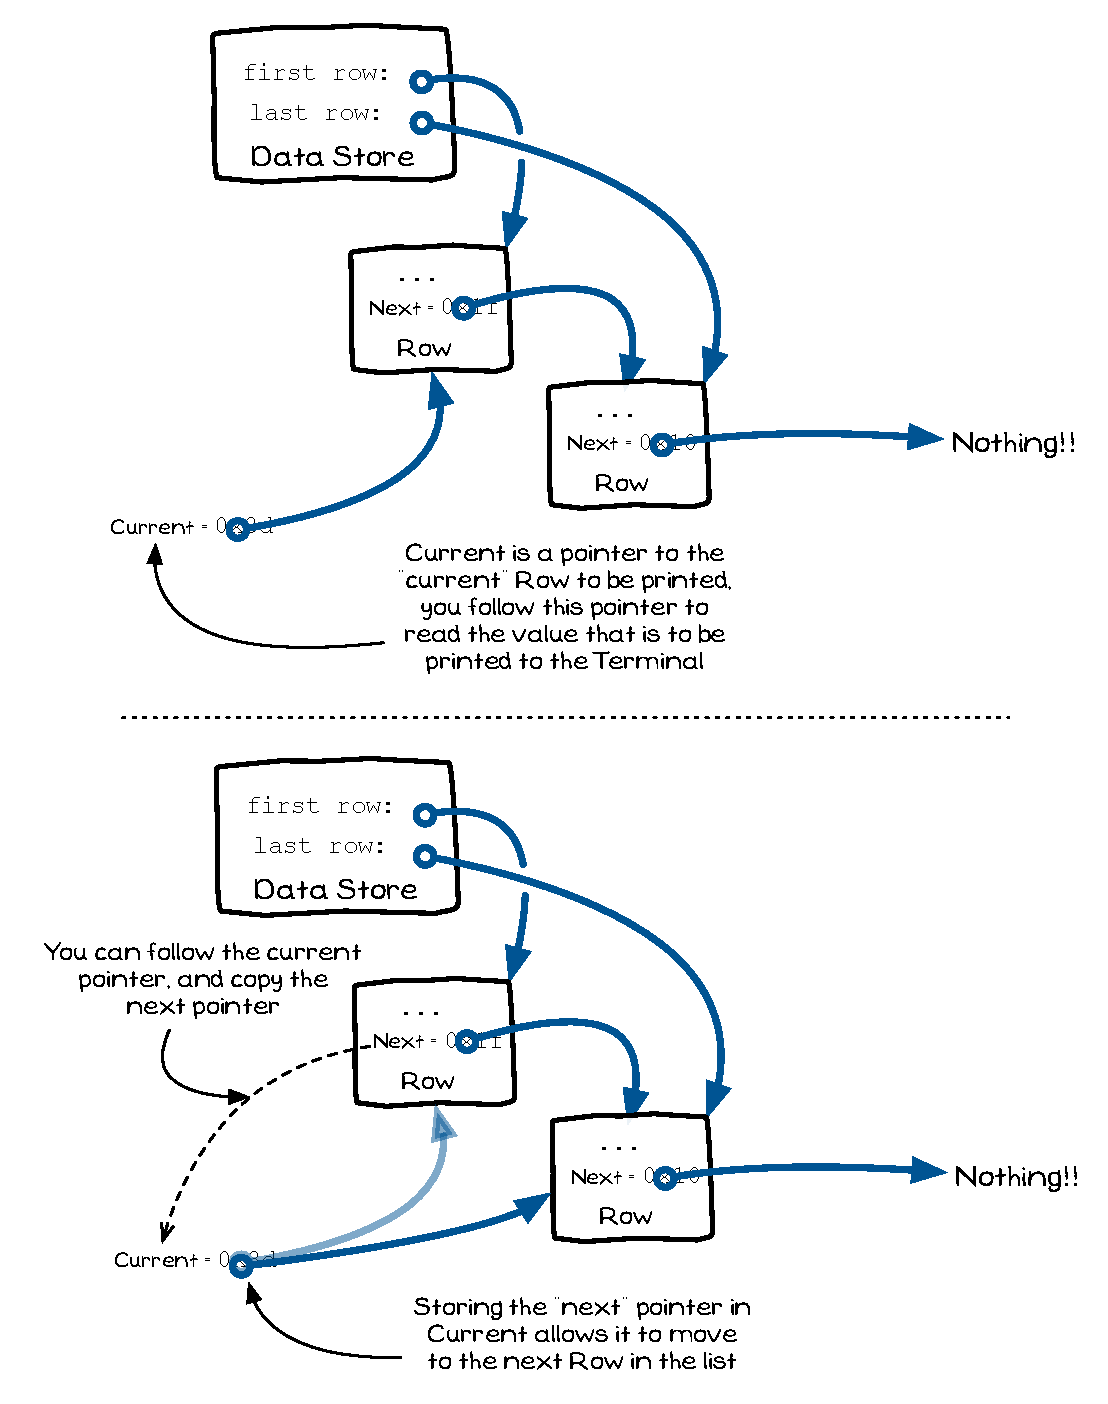
\includegraphics[width=0.75\textwidth]{./topics/dynamic-memory/diagrams/IterateList} 
   \caption{When a new row is added, it becomes the new last row, and the old last node points to it}
   \label{fig:iterate-list}
\end{figure}

\begin{figure}[p]
  \pseudocode{lst:print_all_rows_list}{Pseudocode for the \texttt{Print all Rows} procedure in the linked version of Small DB 2}{topics/dynamic-memory/application/PrintAllNodes.txt}
\end{figure}

\begin{figure}[p]
  \csection{
  \ccode{clst:print_all_rows_list}{C code for \texttt{Print All Rows} procedure in linked version of Small DB 2}{topics/dynamic-memory/application/print-all-rows.c}}
\end{figure}

\begin{figure}[p]
  \passection{
  \pascode{paslst:print_all_rows_list}{Pascal code for \texttt{Print All Rows} procedure in linked version of Small DB 2}{topics/dynamic-memory/application/PrintAllRows.pas}}
\end{figure}

% subsubsection printing_all_rows_in_the_linked_version_of_small_db_2 (end)

\clearpage
\subsubsection{Deleting a row in the linked version of Small DB 2} % (fold)
\label{ssub:deleting_a_row_in_the_linked_version_of_small_db_2}

Deleting a row in the linked version of Small DB 2 will perform much faster than the equivalent array version, as it does not need to copy the array elements. Instead, the deletion of a \texttt{Row} is just a matter of adjusting the links so that the row is no longer included. Though, while it may be faster it will require more thinking and testing as it requires some careful work with pointers.

\fref{fig:delete-row-list} shows an illustration of the actions that need to be coded into the \texttt{Delete a Row} procedure. This code will need to locate the Row to delete, the previous Row, as well as the next Row. When these are located the delete code can change the previous row's \texttt{next} field to be a pointer to the Row that follows the row that is being deleted. With this done the Row has been removed but is still consuming memory. So the last step of this procedure will need to release that memory as it is no longer needed.

The code in \lref{clst:delete_row_list} shows the C code for this process, while the code in \lref{paslst:delete_row_list} shows the matching Pascal code. One key thing to notice is the tracking of the \texttt{prev} \texttt{Row} pointer along with the \texttt{current}. Effectively this is a standard `\emph{for each node}' loop, like that used in \nameref{ssub:printing_all_rows_in_the_linked_version_of_small_db_2}. In this case, the \texttt{prev} pointer remembers the last value of \texttt{current} each time through the loop. This ensures that it will have a pointer to the previous Row when the desired Row is found.

\mynote{
This illustration, and the matching code, only works for nodes in the middle of the list. To fully implement the required functionality you will need to add in a few additional branches that test for the following conditions:
\begin{itemize}
  \item Was a matching Row found? If there is no match then \texttt{current} will point to \emph{Nothing}, and reading \texttt{current}'s \texttt{next} will cause the program to crash.
  \item If the Row is the fist row in the list there will be no previous Row, so \texttt{prev} will point to \emph{Nothing}. Setting \texttt{prev}'s \texttt{next} will cause the program to crash.
  \item Similarly, if the Row is the last row in the list then \texttt{next} will be \emph{Nothing}. This will not cause the program to crash, but will give you errors when you try to add a new node.
\end{itemize}
\medskip
See if you can work out the required logic to address these issues, and implement the full version of this procedure.
}

\begin{figure}[htbp]
   \centering
   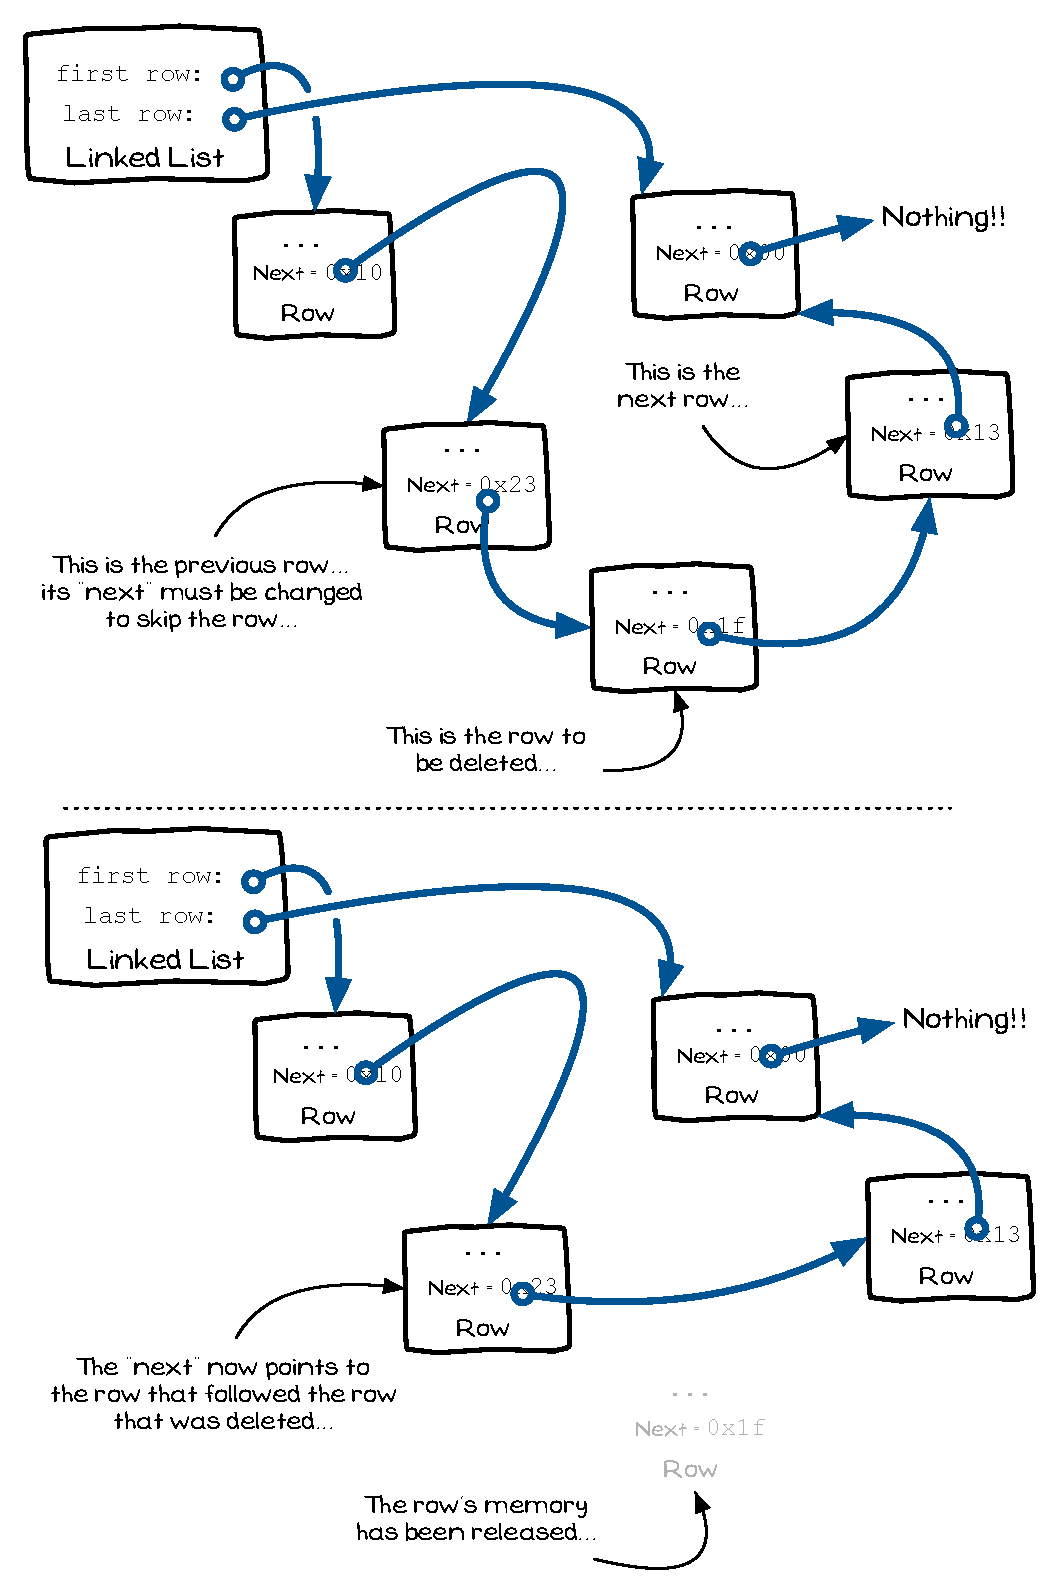
\includegraphics[width=0.9\textwidth]{./topics/dynamic-memory/diagrams/DeleteNode} 
   \caption{When a new row is added, it becomes the new last row, and the old last node points to it}
   \label{fig:delete-row-list}
\end{figure}

\begin{figure}[p]
  \csection{
  \ccode{clst:delete_row_list}{C code for \texttt{Delete a Row} procedure in linked version of Small DB 2}{topics/dynamic-memory/application/delete-row.c}}
\end{figure}

\begin{figure}[p]
  \passection{
  \pascode{paslst:delete_row_list}{Pascal code for \texttt{Delete a Row} procedure in linked version of Small DB 2}{topics/dynamic-memory/application/DeleteRow.pas}}
\end{figure}

% subsubsection deleting_a_row_in_the_linked_version_of_small_db_2 (end)

\subsubsection{Implementing and Testing the linked version of Small DB 2} % (fold)
\label{ssub:implementing_and_testing_the_linked_version_of_small_db_2}

This concludes the design for the linked version of Small DB 2. As you have done in the past you will need to work out how to code this using the syntax diagrams and examples from hhe following two sections: \sref{sec:dynamic_memory_allocation_in_c} \nameref{sec:dynamic_memory_allocation_in_c} and  \sref{sec:dynamic_memory_allocation_in_pascal} \nameref{sec:dynamic_memory_allocation_in_pascal}. 

During the implementation process you should also be testing your solution. With pointers, as with anything, it is best to write a little and then test it. Use the same testing strategy as discussed in  \nameref{ssub:the_testing_phase_compiling_and_running_small_db_2}. This should help you locate any memory issues with this code.

\mynote{
As this code requires more work with pointers you are likely to have more issues. You should expect your program to crash a few times as you work through these, so do not worry if this does happen. The best way to work through these issues is with a piece of paper and a pencil. Use this to draw up the different \texttt{Row} values and their pointers. Then work through the actions yourself on paper.
}
% subsubsection implementing_and_testing_the_linked_version_of_small_db_2 (end)

% subsection the_design_place_designing_linked_small_db_2 (end)

